
\chapter{Methodology}

\section{Solution Proposal}

We present our proposed solution for the acoustic inspection of metal structures using multi-robot navigation strategies.
We have developed three specific strategies to optimize data acquisition and enable the tomography of metallic surfaces.
These three strategies are:
\begin{enumerate}
	\item \textit{Roller Painting} navigation strategy
	\item \textit{Nordic Skiing} navigation strategy
	\item \textit{Polygonal Investigation} navigation strategy
\end{enumerate}
Among these strategies, the first two are non-reactive and can be considered as coarse exploration strategies, the goal being to quickly obtain a global coverage of the surface to be inspected.
The third strategy is reactive and makes it possible to optimize the acquisition of data for the realization of the tomography.
These three strategies aim to map the metal surface and detect areas of corrosion.
We define these three navigation strategies in the following subsections.
We also explain how the data structure used for mapping corrosion areas, an occupancy grid, is updated based on information collected by the robots' \gls{ugw} sensors.

\subsection{Occupancy Grid Update Process for Mapping}

When scanning the surface to be inspected by a pair of transmitter and receiver robots, the transmitter robot emits an acoustic wave in the metal structure, which is then received by the receiver robot.
The detection being considered as perfect, the receiver robot receives the wave emitted by the transmitter robot, without quasi-alteration of the power of the signal, if and only if the line segment between the two robots does not cross a zone of corrosion.
It is thus possible to determine whether a corrosion zone is present between the two robots by checking whether the signal received by the receiving robot is sufficiently powerful.
Insofar as there is no detection of corrosion between the transmitter and the receiver, then the line segment between the two robots is considered to be free of corrosion.
Otherwise, then the points of the line segment between the two robots are considered to be corrosion, with the exception of the points previously perceived to be free of corrosion.
The presence of corrosion on the segment is therefore overestimated.
The displacement strategies will aim to carry out several measurements, to reduce this overestimation, and approach the real shape of the corrosion.

We now only need to determine which cells of the occupancy grid are crossed by the line segment between the two robots.
For this we use Bresenham's segment drawing algorithm~\cite{enwiki:1155124335} which is commonly used to determine the points of a discrete plane that need to be drawn in order to form an approximation of a line segment between two given points.
We detail our implementation of this algorithm in \ref{subsec:Bresenham}.

As the metal surface is explored, the occupation grid is updated based on the information gathered by the robots.
More precisely, the cells of the occupancy grid that identify corrosion elements are updated with the occupied state, while the cells that identify healthy areas are updated with the empty state.
We thus end up with an occupation grid which represents the state of corrosion of the metal surface, with, for each corrosion zone, an approximation of the convex envelope of the corrosion zone.

\subsection{\textit{Roller Painting} Navigation Strategy}

The first navigation strategy we propose is the \textit{Roller Painting} navigation strategy.
We chose this name for this strategy because the movement of the robots during this strategy is similar to that of a paint roller when painting a wall.
This strategy is based on a rough exploration of the surface to be inspected, where the robots move in a straight line on parallel trajectories, guaranteeing global coverage of the inspection area.
It is therefore a question here of carrying out a grid of the surface to be inspected.

\begin{figure}[h!]
	\centering
	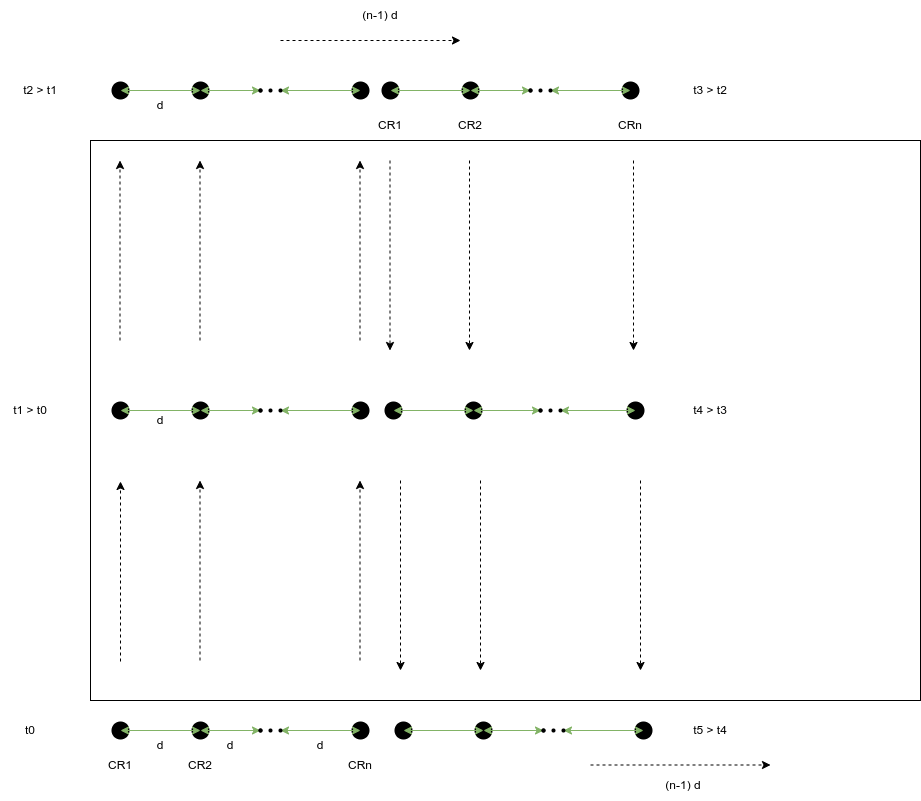
\includegraphics[scale=0.45]{graphics/peinture_au_rouleau.png}
	\caption{\textit{Roller Painting} navigation strategy - vertical phase.}
	\label{fig:peinture_au_rouleau}
\end{figure}

We present in \ref{fig:peinture_au_rouleau} a diagram describing the paint roller navigation strategy.
This strategy consists of two phases, a vertical movement phase and a horizontal movement phase.
The \ref{fig:peinture_au_rouleau} shows the first phase of vertical displacement.
In order to achieve this strategy, a minimum of $n \in \mathbb{N}$ robots, $n \ge 2$, aligned horizontally and separated by a distance $d < d_{max}$, is used.
These robots move vertically, simultaneously, following a parallel trajectory.
Once the end of the surface to be inspected has been reached, the robots rotate 90 degrees and move horizontally, simultaneously, by a distance $(n - 1) \cdot d$.
They then perform a new 90 degree rotation and move again vertically, in a straight line, simultaneously, following a path parallel to each other, until they reach the other end of the surface to be inspected.
This process is repeated until the metal surface is fully inspected.
The same process is then repeated, but this time horizontally.

During this strategy, each robot is both a transmitter and a receiver of \gls{ugw}s.
If the distance separating a robot $n_a$ from a robot $n_b$, $(n_a, n_b) \in \{1, 2, \dots, n\}^2$, is less than the maximum propagation distance of the \gls{ugw}s, $d_{max}$, then the robot $n_a$ is able to receive the signal emitted by the robot $n_b$ and vice versa.
However, it is not necessary for a robot $n_k$, $n_k \in \{1, 2, \dots, n\}$, to process signals received from all other robots.
Indeed, the robots being aligned, the signals received from the robots $n_{k-1}$ and $n_{k+1}$, are sufficient for the reconstruction of the state of the metallic surface.
The waves emitted by the robots $n_1, n_2, \dots, n_{k-2}$ and $n_{k+2}, \dots, n_n$ are not useful for the robot $n_k$.
The robot $n_k$ can therefore ignore these signals and concentrate only on the signals received from the robots $n_{k-1}$ and $n_{k+1}$.
Insofar as the first signals perceived by the robot $n_k$ are those emitted by the robots $n_{k-1}$ and $n_{k+1}$, due to their proximity, it is possible for the robot $n_k$ to filter signals received from other robots.
This constitutes an optimization in terms of processing for each robot.

The fact that the robots move along a parallel trajectory and simultaneously, implies that the rays of the signal emitted by the transmitter robot and received by the receiver robot, always have an orientation of $0$ radian for the vertical phase and an orientation of $\frac{\pi}{2}$ radians for the horizontal phase.
There is therefore not a large variation in the orientation of the transmitted and received signal.
Thus, this strategy will only be able to approach the convex envelopes of the corrosion zones by rectangles.
Examples of occupancy grids resulting from the \textit{Roller Painting} navigation strategy, represented as images, where the cells of the grid correspond to the pixels of the images, are shown in \ref{annexe:resultat}, \ref{fig:peinture_au_rouleau_resultats}.

\subsection{\textit{Nordic Skiing} Navigation Strategy}

The second strategy we propose is the navigation strategy \textit{Nordic Skiing}.
We chose this name for this strategy because the movement of the robots during this strategy is similar to the movement of a skier's skis.
This strategy still consists of moving in a straight line and following parallel trajectories, but this time the robots move sequentially and no longer simultaneously.
In this strategy, we wanted to increase the orientation diversity of the transmitted and received signal rays, in order to approach more precisely the convex envelopes of the corrosion zones.

\begin{figure}[h!]
	\centering
	\begin{subfigure}[t]{0.45\linewidth}
		\centering
		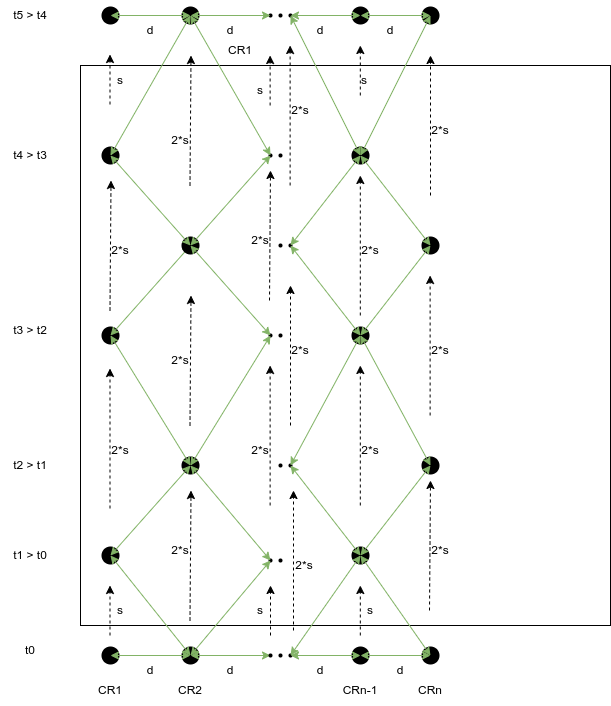
\includegraphics[width=\linewidth]{graphics/ski_nordique_1.png}
		\caption{\textit{Nordic Skiing} navigation strategy - first phase.}
		\label{fig:ski_nordique_1}
	\end{subfigure}
	\hfill
	\begin{subfigure}[t]{0.45\linewidth}
		\centering
		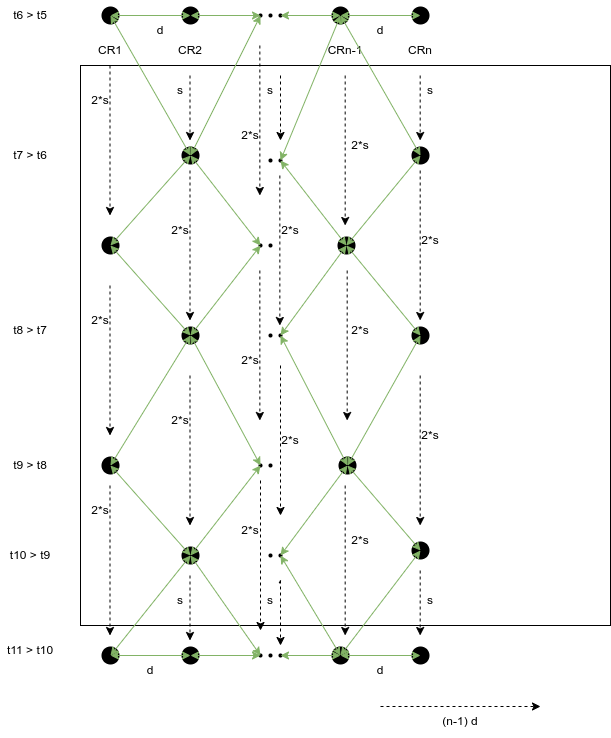
\includegraphics[width=\linewidth]{graphics/ski_nordique_2.png}
		\caption{\textit{Nordic Skiing} navigation strategy - second phase.}
		\label{fig:ski_nordique_2}
	\end{subfigure}
	\caption{\textit{Nordic Skiing} navigation strategy - vertical phase.}
	\label{fig:ski_nordique}
\end{figure}

\ref{fig:ski_nordique} presents a diagram describing the \textit{Nordic Skiing} navigation strategy.
This strategy also consists of two phases, a vertical movement phase and a horizontal movement phase.
\ref{fig:ski_nordique} shows the first phase of vertical movement.
In order to achieve this strategy, a minimum of $n \in \mathbb{N}$ robots, $n \ge 2$, aligned horizontally and separated by a distance $d < d_{max}$, is used.
These robots move vertically, following a parallel path, but sequentially.
The odd robots move in a straight line a distance $s$ and stop.
The even robots then move in a straight line a distance of $2 \cdot s$ and stop.
This process is repeated until the end of the surface is reached (\ref{fig:ski_nordique_1}).
Then, the robots repeat this same process, in the opposite direction and so that the stopping points of the robots are not the same as those previously (\ref{fig:ski_nordique_2}).
That is to say that this time, it is the even robots which start by moving in a straight line for a distance $s$ and then stop.
Then the odd robots move in a straight line for a distance of $2 \cdot s$ and then stop.
The robots then move horizontally a distance $(n - 1) \cdot d$ and repeat the same process until the metal surface is fully inspected.
The same process is then repeated, but this time horizontally.
In order for the various receiver robots to be able to receive the signals emitted by the transmitter robots, it is also necessary to impose that $s$ be strictly less than $\frac{d_{max}}{2}$, i.e. $s < \frac{d_ {max}}{2}$.

During this strategy, each robot is both a transmitter and a receiver of \gls{ugw}s.
Here, as with the \textit{Roller Painting} navigation strategy, it is not necessary for a robot $n_k$, $n_k \in \{1, 2, \dots, n\}$, to process the signals received by robots other than $n_{k-1}$ and $n_{k+1}$.

The fact that the robots move following a parallel trajectory, but in a sequential way, implies that the rays of the signal emitted by the transmitter robot and received by the receiver robot, have an orientation of greater variation.
Thus, this strategy makes it possible to approximate the convex envelopes of the corrosion zones by more diverse and precise shapes than rectangles.
Examples of occupation grids resulting from the \textit{Nordic Skiing} navigation strategy, represented in the form of images, where the cells of the grid correspond to the pixels of the images, are shown in \ref{annexe:resultat}, \ref{fig:ski_nordique_resultats} and \ref{fig:ski_nordique_resultats_2}.

\subsection{\textit{Polygonal Investigation} Navigation Strategy}

The third strategy we propose is the \textit{Polygonal Investigation} navigation strategy.
We have seen, previously, that at the end of the realization of the \textit{Roller Painting} navigation strategy, the convex envelope of the corrosion zones was approximated by a rectangle.
This approximation is a little more precise for the \textit{Nordic Skiing} navigation strategy.
It would be interesting to have a greater degree of precision around potential areas of corrosion.
This is what we propose with the \textit{Polygonal Investigation} navigation strategy.
This strategy consists of investigating around potential areas of corrosion, previously detected by one of the two previous navigation strategies.
It consists of positioning the robots around the corrosion zones and making them move along a polygonal trajectory, so that the rays of the signal emitted and received have an orientation of greater variation even around these zones.

\begin{figure}[h!]
	\centering
	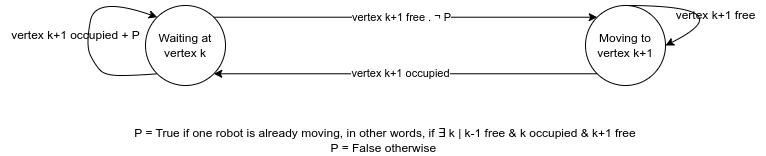
\includegraphics[scale=0.6]{graphics/automat_poly.png}
	\caption{\textit{Polygonal Investigation} navigation strategy.}
	\label{fig:automat}
\end{figure}

We present in \ref{fig:automat} a finite state automaton describing the \textit{Polygonal Investigation} navigation strategy.
At the beginning of the \textit{Polygonal Investigation} navigation strategy, each $n \in \mathbb{N}$ robots, $n \ge 2$, of $k \in \mathbb{N}$ teams, $k \ge 1$, are positioned on consecutive vertices of a polygon $P$ with $p \in \mathbb{N}$ vertices, $p \ge 3$, enclosing the potential area of corrosion.
To ensure the proper functioning of the strategy, it is necessary that the distance $d^*$, corresponding to the maximum distance between two vertices of the polygon $P$, be strictly less than $d_{max}$, i.e. $d^* < d_{max}$.
In the latter, each robot has two states.
The first consists of waiting and the second consists of moving along the polygonal trajectory, namely traversing the various vertices that make up the polygon.
The robot capable of advancing, that is to say, whose next vertex is not occupied by another robot, advances.
The others wait until the advancing robot reaches the last free vertex of the polygon.
The process is then repeated for each robot of each team until the vertices occupied by the robots are the same as those occupied at the beginning of the \textit{Polygonal Investigation} navigation strategy.

\begin{figure}[h!]
	\centering
	\begin{subfigure}[t]{0.27\linewidth}
		\centering
		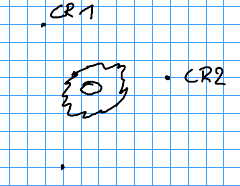
\includegraphics[width=\linewidth]{graphics/triangle_1.png}
		\caption{Initial phase, crawlers are positioned on consecutive vertices of the polygon.}
		\label{fig:triangle_1}
	\end{subfigure}
	\hfill
	\begin{subfigure}[t]{0.27\linewidth}
		\centering
		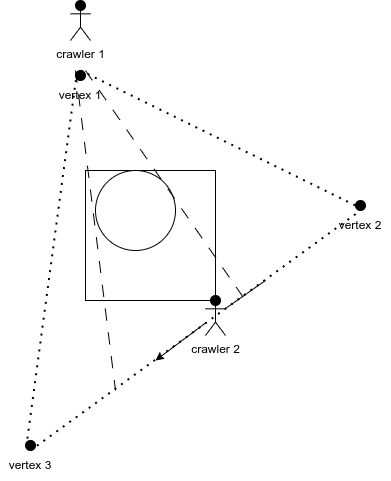
\includegraphics[width=\linewidth]{graphics/triangle_2.png}
		\caption{First phase of movement, crawler 2 moves from vertex 2 to vertex 3.}
		\label{fig:triangle_2}
	\end{subfigure}
	\hfill
	\begin{subfigure}[t]{0.27\linewidth}
		\centering
		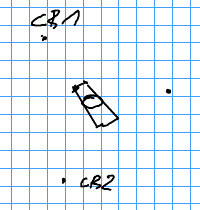
\includegraphics[width=\linewidth]{graphics/triangle_3.png}
		\caption{Second phase, crawler 2 reaches vertex 3 and stops.}
		\label{fig:triangle_3}
	\end{subfigure}
	\hfill
	\begin{subfigure}[t]{0.27\linewidth}
		\centering
		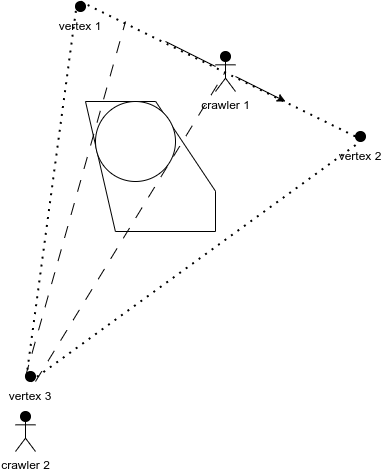
\includegraphics[width=\linewidth]{graphics/triangle_4.png}
		\caption{Second phase of movement, crawler 1 moves from vertex 1 to vertex 2.}
		\label{fig:triangle_4}
	\end{subfigure}
	\hfill
	\begin{subfigure}[t]{0.27\linewidth}
		\centering
		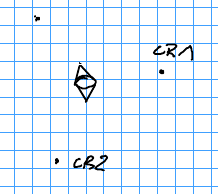
\includegraphics[width=\linewidth]{graphics/triangle_5.png}
		\caption{Third phase, crawler 1 reaches vertex 2 and stops.}
		\label{fig:triangle_5}
	\end{subfigure}
	\hfill
	\begin{subfigure}[t]{0.27\linewidth}
		\centering
		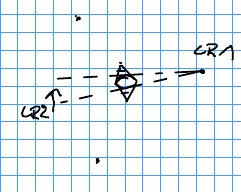
\includegraphics[width=\linewidth]{graphics/triangle_6.png}
		\caption{Third phase of movement, crawler 2 moves from vertex 3 to vertex 1.}
		\label{fig:triangle_6}
	\end{subfigure}
	\hfill
	\begin{subfigure}[t]{0.27\linewidth}
		\centering
		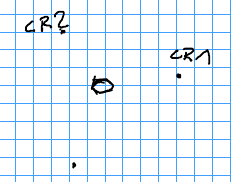
\includegraphics[width=\linewidth]{graphics/triangle_7.png}
		\caption{Last phase, crawler 2 reaches vertex 1 and stops.}
		\label{fig:triangle_7}
	\end{subfigure}
		\caption{Movement phases of the \textit{Polygonal Investigation} navigation strategy.}
		\label{fig:triangle}
\end{figure}

We present in \ref{fig:triangle} an example of the different moving phases of the \textit{Polygonal Investigation} navigation strategy with $k = 1$ team, $n = 2$ robots and $p = 3$ vertices.
On these different figures, we have represented a corrosion zone by a circle and an approximation of this zone by a square enveloping the circle, as we can see in \ref{fig:triangle_1}.
The objective is to approach the corrosion zone as finely as possible.
The corrosion zone is not known in advance, only the shape of the square enveloping the circle is known.
\ref{fig:triangle_1} presents the initial phase of the \textit{Polygonal Investigation} navigation strategy, where the two crawlers are positioned on consecutive vertices of the polygon.
\ref{fig:triangle_2} shows the first moving phase of the \textit{Polygonal Investigation} navigation strategy, while the crawler 2 moves from vertex 2 to vertex 3, until it reaches the latter, as we can see in \ref{fig:triangle_3}.
We can see that after the crawler 2 has reached vertex 3, part of the suspected corrosion area is removed and considered healthy, as we can see in \ref{fig:triangle_3}.
The crawlers keep moving until they reach their initial position, as we can see in \ref{fig:triangle_7}.

\begin{definition}[Phantom zone]
	\label{def:fantomas}
	A phantom zone is a corrosion zone detected by one of the navigation strategies, but which is not a corrosion zone. It is a false positive.
\end{definition}

The \textit{Polygonal Investigation} navigation strategy has two advantages.
The first is that it quickly eliminates phantom zones (\ref{def:fantomas}).
The second is that it makes it possible to approach the convex envelopes of the corrosion zones by more diverse and precise shapes than rectangles due to the great variation in the orientation of the rays of the signal emitted and received by the robots around each vertex of the polygon.

This strategy requires two steps prior to its execution:
\begin{enumerate}
	\item the extraction of the corrosion zones detected by one of the preceding navigation strategies.
	\item determining the order of investigation of corrosion areas.
\end{enumerate}

The first step can be solved using a \gls{scc} graph decomposition algorithm.
A \gls{scc} is defined in \ref{def:scc}.
We then consider our occupation grid, resulting from the exploration of one of the two previously defined strategies, as an undirected graph $G = (V, E)$, where $V$ is the set of vertices of the graph, corresponding to the cells of the occupancy grid and $E$ is the set of edges of the graph, corresponding to the adjacent cells of the occupancy grid.
This problem is well known and there are simple algorithms to solve it, such as Tarjan's algorithm~\cite{enwiki:1148118528}, of linear time complexity $O(|V| + |E|)$.
We will not look further into this problem and entrust its resolution to the \textit{OpenCV} library.

\begin{definition}[\gls{scc}]
	\label{def:scc}
	A strongly connected component of a graph $G = (V, E)$ is a subset $C$ of $V$ such that for any pair of vertices $(u, v) \in C^2$, there is a path from $u$ to $v$ and a path from $v$ to $u$.
\end{definition}

\begin{definition}[Hamiltonian cycle]
	\label{def:hamilton}
	A Hamiltonian cycle is a cycle passing through all the vertices of a graph, once and only once.
\end{definition}

\begin{definition}[\gls{tsp}]
	\label{def:tsp}
	Given a graph $G = (V, E)$, where $V$ is the set of vertices of the graph and $E$ is the set of edges of the graph, and a cost function $c : E \rightarrow \mathbb{R}$, the \gls{tsp} consists in finding a Hamiltonian cycle (\ref{def:hamilton}) of minimal cost in $G$.
\end{definition}

\begin{definition}[Multi-depot \gls{mtsp}]
	\label{def:mtsp}
	Given a graph $G = (V, E)$, where $V$ is the set of vertices of the graph and $E$ is the set of edges of the graph, a cost function $c : E \rightarrow \mathbb{R}$, and a set of depots $D \subset V$, the multi-depot \gls{mtsp} is to find a set of cycles of minimum total cost in $G$, each going through one and only one deposit.
\end{definition}

The second step can be solved using a \gls{tsp} (\ref{def:tsp}) algorithm in the case where the number of teams $k$ is equal to 1 and a \gls{mtsp} (\ref{def:mtsp}) algorithm in the case where the number of teams $k$ is strictly greater than 1.
There are several solution paradigms to solve this type of problem.
A first is to find an exact solution using an integer linear programming algorithm.
A second is to find an approximate solution using a meta-heuristic.

\begin{definition}[\gls{np} Class]
	\label{def:np}
	The class \gls{np} is the class of decision problems that can be solved by a non-deterministic algorithm in polynomial time.
\end{definition}

\begin{definition}[\gls{np}-hard problem]
	\label{def:nph}
	A problem is \gls{np}-hard if it is at least as hard as problems of class \gls{np}.
	In other words, a problem is \gls{np}-hard if there is a polynomial reduction algorithm that transforms a problem of class \gls{np} into an instance of this problem.
\end{definition}

\begin{definition}[\gls{np}-complete problem]
	\label{def:npc}
	A problem is \gls{np}-complete if it is both \gls{np} and \gls{np}-hard.
\end{definition}

The \gls{tsp} is a \gls{np}-complete (\ref{def:npc}) problem.
It can be treated as an integer linear optimization problem~\cite{article244, gurobi25}.
To do this, we use the formulation presented in \ref{eq:tsp}.

\begin{equation}
	\label{eq:tsp}
	\begin{array}{ll@{}rr}
		\text{minimize} &
		\displaystyle\sum\limits_{i \in V} \sum\limits_{j \in V} c_{ij} x_{ij} &
		&
		\\
		\text{subject to} &
		\displaystyle\sum\limits_{i \in V} x_{ij} = 1 &
		&
		\forall j \in V \\
		&
		\displaystyle\sum\limits_{j \in V} x_{ij} = 1 &
		&
		\forall i \in V \\
		&
		\displaystyle\sum\limits_{i \in S} \sum\limits_{j \in S} x_{ij} \leq |S| - 1 &
		&
		\forall S \subset V, 2 \leq |S| \leq |V| - 1 \\
		&
		x_{ij} \in \{0, 1\} &
		&
		\forall i \in V, \forall j \in V \\
	\end{array}
\end{equation}

The objective function to be minimized from the \ref{eq:tsp} is the sum of the distances between each pair of locations.
The first two constraints ensure that each city is visited exactly once.
The third constraint ensures that the cycle formed by the cities visited is simple, that is to say, that it does not contain sub-cycles.
The last constraint ensures that the decision variables $x_{ij}$ are binary, with $x_{ij} = 1$ if the robot moves from city $i$ to city $j$ and $x_{ij} = 0$ otherwise.

The \gls{mtsp} is an \gls{np}-hard problem (\ref{def:nph})~\cite{SUNDAR201639}.
This one can be solved using meta-heuristics like a genetic algorithm~\cite{SinghMTSP, Kiraly2011}

In the next sections, we will detail each navigation strategy, exposing the specific algorithms and mechanisms used to implement our proposed solution. We will also analyze the performance and results obtained through extensive experimentation and evaluation.

\section{Algorithm Implementations}

In this section, we highlight some of the different technical implementations we have developed to support our multi-robot navigation and control solutions in the context of acoustic inspection of metal structures.
We begin by describing our adaptation of Bresenham's line algorithm~\cite{enwiki:1155124335}, widely used to determine which points of a discrete plane should be plotted in order to form a segment approximation of line between two given points.
Next, we discuss the implementation of the \textit{Roller Painting} algorithm, which allows the robots to move simultaneously, following parallel trajectories.
We continue with the implementation of the \textit{Nordic Skiing} algorithm, which allows the robots to move alternately, following parallel trajectories, thus modifying the orientation of the vector representing the direction of movement of the wave transmitted and received by the pair of robots.
Additionally, we look at the implementation of the \textit{Polygonal Investigation} algorithm, which allows robots to examine suspected areas of corrosion more precisely.
Finally, we present Cohen's $\kappa$ algorithm~\cite{enwiki:1130024730}, used to assess the quality and reliability of the acoustic inspection results.
We discuss in detail our implementation of this algorithm, which provides quantitative measures to evaluate the performance of robots in the inspection of metal structures.
Each of these technical implementations contributes to the efficiency and accuracy of our multi-robot navigation and control approach, and will be discussed in detail in the following subsections.

\subsection*{Bresenham's Line Algorithm}\label{subsec:Bresenham}

\begin{algorithm}[h!]
	\caption{Process of updating the occupancy grid using Bresenham's line algorithm.}
	\label{alg:Bresenham}
	\KwData{$P_1 \in \mathbb{R}^2$, $P_2 \in \mathbb{R}^2$, $pw \in \mathbb{R}$, $threshold \in \mathbb{R}$, $G$: $l \times w \rightarrow [\text{UNKNOWN}, \text{EMPTY}, \text{OCCUPIED}]$, $l \in \mathbb{N}$, $w \in \mathbb{N}$ \\
		with $P_1$ and $P_2$ the two points to connect, $pw$ the power of the \gls{ugw}, $threshold$ the threshold above which the power of the \gls{ugw} is considered undistributed and $G$ the grid to update.}
	\KwResult{The updated grid.}
	$p_0 \gets \text{from\_position\_to\_grid\_coordinate}(P_1)$ \\
	$p_1 \gets \text{from\_position\_to\_grid\_coordinate}(P_2)$ \\
	\If{\text{is\_out\_of\_grid}($p_0$) \textbf{or} \text{is\_out\_of\_grid}($p_1$)}{
		\Return
	}
	$dx \gets p_1.x - p_0.x$ \\
	$dy \gets p_1.y - p_0.y$ \\
	$sx \gets \text{sign}(dx)$ \\
	$sy \gets \text{sign}(dy)$ \\
	$err = dx - dy$ \\
	\While{$p_0 \neq p_1$}{
		\If{$pwd \leq threshold$ \textbf{and} $G(p_0) = \text{UNKNOWN}$}{
			$G(p_0) \gets \text{OCCUPIED}$
		}
		\ElseIf{$pwd > threshold$}{
			$G(p_0) \gets \text{EMPTY}$
		}
		$e2 \gets 2 \times err$ \\
		\If{$e2 > -dy$}{
			$err \gets err - dy$ \\
			$p_0.x \gets p_0.x + sx$
		}
		\If{$e2 < dx$}{
			$err \gets err + dx$ \\
			$p_0.y \gets p_0.y + sy$
		}
	}
\end{algorithm}

We use Bresenham's line algorithm to determine the points of the line segment between the two robots.
The algorithm is presented in \ref{alg:Bresenham}.
The part adapted to our problem is between lines 12 and 17 of the latter.
At this point, we check if the signal strength is sufficiently impaired and if the point of the line segment between the two robots has not already been perceived as free of corrosion.
If so, then the considered point is marked as corrosion, modeled by the value \texttt{OCCUPIED}.
If the signal strength is not sufficiently altered, then the considered point is marked as being free of corrosion, modeled by the value \texttt{EMPTY}.
Once all the points of the segment have been traversed, the grid $G$ is updated with the new information.
Bresenham's line algorithm thus contributes to the construction of the occupation grid which makes it possible to locate the corrosion zones detected by the robots during the acoustic inspection of metal structures.

\subsection*{\textit{Roller Painting} and \textit{Nordic Skiing} Algorithms}

We present in this subsection the implementations of the \textit{Roller Painting} and \textit{Nordic Skiing} algorithms.
Their source code is available on GitLab, here\footnote{\url{https://gitlab.georgiatech-metz.fr/bugwright2/bugwright2-ws/blob/cr_nav_strat/bugwright_ws/src/floor_nav/missions/peinture_au_rouleau.py}} and here\footnote{\url{https://gitlab.georgiatech-metz.fr/bugwright2/bugwright2-ws/blob/cr_nav_strat/bugwright_ws/src/floor_nav/missions/ski_nordique.py}}.

The implementations of these algorithms have been made using the Python programming language and the \gls{ros} libraries.
In these implementations, we use the \gls{ros} Task Manager~\cite{ROSTaskManager} framework to manage the tasks of the robot inspectors.
First, we initialize the \gls{ros} node and create a task client.
Then, we retrieve the necessary parameters such as the speed of the crawlers, the crawler identifier, the distance between the crawlers, the overlap or the dimensions of the surface to be inspected.

The algorithms are then executed following a sequence of precise movements.
For each crawler, we define vertical and horizontal trajectories using an iterative loop and mathematical calculations.
Crawlers move along defined paths, using task client functions such as \texttt{AlignWithTarget} and \texttt{FollowLine} to maintain a precise path.

During the execution of the algorithms, the crawlers synchronize using the \texttt{SetStatusSync} and \texttt{WaitForStatusSync} functions of the task client.
This ensures that the crawlers perform the movements in a coordinated manner and position themselves correctly to cover the entire metal surface.
At the end of each movement step, the status is updated and synchronization is performed with the corresponding partner.

The implementation of the two algorithms \textit{Roller Painting} and \textit{Nordic Skiing} allow crawlers to explore the metal surface in a methodical and complete way.
Using vertical and horizontal trajectories, crawlers traverse the surface overlapping previously inspected areas to ensure optimal coverage.
Here we have used a 10 cm overlap between the different vertical and horizontal trajectories.

Once the algorithms are completed, the execution time is recorded, providing an indication of how long it took to inspect the metal surface.
The occupancy grid is also recorded in order to calculate the inspection score.
This implementation is an essential step in our proposed solution for the acoustic inspection of metal structures and guarantees complete and effective coverage of the surface to be inspected.

\subsection*{\textit{Polygonal Investigation} Algorithm}

We present in this subsection the implementation of the \textit{Polygonal Investigation} algorithm.
The corresponding source code is available on GitLab~\footnote{\url{https://gitlab.georgiatech-metz.fr/bugwright2/bugwright2-ws/blob/cr_nav_strat/bugwright_ws/src/floor_nav/missions/investigation_polygonale.py}} .

The implementation of this algorithm was also carried out using the Python programming language and the \gls{ros} libraries.
In this implementation, we still use the \gls{ros} Task Manager~\cite{ROSTaskManager} framework to manage the tasks of the inspector robots.
First, we initialize the \gls{ros} node and retrieve the different parameters and more particularly the map of potential corrosion zones, on which we base ourselves for the inspection, which come from one of the two coarse strategies.
Next, we extract the \gls{scc} from the map using the \texttt{connectedComponentsWithStats} function from the \textit{OpenCV} library.
This function uses Bolleli's spaghetti algorithm~\cite{BolelliSpaghetti} to extract \gls{scc} from an image.
For each of these components, we retrieve its center and its dimensions.
Next, we construct a $p \in \mathbb{N}$ sided polygon around each center of a component.
To do this, we place $p$ points on an ellipse centered on the center of the component and whose axes are the dimensions of the component.
We therefore have for each potential zone of corrosion a polygon with $p$ sides which surrounds it.
All that remains is to find the shortest path that passes through all the polygons.
For this, we use the \textit{Gurobi} library to solve a simple \gls{tsp} in the case where the number of teams of robots $k = 1$.
When $k > 1$, we use the genetic algorithm proposed by Elad Kivelevitch~\cite{MDMTSPV_GA} to solve the multi-depot \gls{mtsp}.

Once the algorithms are completed, the run time is recorded, providing an indication of how long it will take to inspect the various potential areas of corrosion.
The occupancy grid is also recorded in order to calculate the inspection score.
This implementation is an essential step in our proposed solution for the acoustic inspection of metal structures and allows us to investigate potential areas of corrosion in an efficient way.

\subsection*{Algorithm for Calculating Cohen's $\kappa$}

Assessing the quality and reliability of acoustic inspection results is essential to ensure accurate measurements of the condition of metal structures.
In this subsection, we present the algorithm for calculating Cohen's $\kappa$~\cite{enwiki:1130024730}, introduced in \ref{alg:Cohen_Kappa}, a statistical measure commonly used to assess the agreement between the results obtained by the robots and a human reference.

\begin{table}[h!]
	\centering
	\begin{tabular}{|c|c|}
		\hline
		$\kappa$ & Interpretation \\
		\hline
		$< 0$ & Disagreement \\
		\hline
		$0.00 - $0.20 & Very Low agreement \\
		\hline
		$0.21 - $0.40 & Low agreement \\
		\hline
		$0.41 - $0.60 & Moderate agreement \\
		\hline
		$0.61 - $0.80 & Strong agreement \\
		\hline
		$0.81 - $1.00 & Almost perfect agreement \\
		\hline
	\end{tabular}
	\caption{Interpretation of Cohen's $\kappa$ according to Landis and Koch.}
	\label{tab:Kappa_Cohen}
\end{table}

Cohen's $\kappa$ calculation algorithm is based on the notion of concordance and discordance between the results of inspections carried out by robots and those carried out by human inspectors (ground truth).
It takes into account the positive, negative, false positive and false negative results obtained during the acoustic inspection.
This information is used to calculate the value of the Cohen coefficient, noted $\kappa$, with $\kappa = \frac{p_o - p_e}{1 - p_e}$, where $p_o$ is the observed rate of agreement and $p_e$ the expected agreement rate.

\begin{algorithm}[h!]
	\caption{Cohen's $\kappa$ algorithm.}
	\label{alg:Cohen_Kappa}
	\KwData{$I_0$: $l \times w \times 3 \rightarrow [0 .. 255]$, $I$: $l \times w \times 3 \rightarrow [0 .. 255]$, $l \in \mathbb{N}$, $w \in \mathbb{N}$ \\
		with $I_0$ the ground truth image and $I$ the image to score.}
	\KwResult{$\kappa \in [0, 1]$}
	$TP \gets 0$ \\
	$TN \gets 0$ \\
	$FP \gets 0$ \\
	$FN \gets 0$ \\
	\For{$i \gets 1$ \KwTo $l$}{
		\For{$j \gets 1$ \KwTo $w$}{
			\If{$\text{is\_label\_1}(I_0(i, j))$}{
				\If{$\text{is\_label\_1}(I(i, j))$}{
					$TP \gets TP + 1$
				}
				\Else{
					$FN \gets FN + 1$
				}
			}
			\Else{
				\If{$\text{is\_label\_1}(I(i, j))$}{
					$FP \gets FP + 1$
				}
				\Else{
					$TN \gets TN + 1$
				}
			}
		}
	}
	$f_c \gets \frac{(TN + FN) (TN + FP) + (FP + TP) (FN + TP)}{TP + TN + FN +FP}$ \\
	$\kappa \gets \frac{TP + TN - f_c}{TP + TN + FN + FP - f_c}$
\end{algorithm}

The algorithm proceeds in several steps.
First, the results of the inspections carried out by the robots and the actual distributions of the corrosion zones are compared for each zone inspected.
To do this, we compare the values of each cell of the occupancy grid, obtained at the end of the inspection by the robots, with those of the ground truth.
Having modeled the different test environments, we know the true distribution of the corrosion zones.
Then, the results are grouped into four categories: positive agreement, negative agreement, positive discrepancy (false positives), and negative discrepancy (false negatives).
These categories are used to calculate the observation and agreement rates observed between the robots and the true distribution of the corrosion zones.
Cohen's $\kappa$ is then calculated from observed observation and agreement rates, taking into account the possibility of concordance due to chance.
The closer Cohen's $\kappa$ is to 1, the greater the agreement between the robot results and the ground truth results.
On the other hand, a $\kappa$ close to 0 indicates a low level of agreement, while a negative $\kappa$ suggests a discrepancy between the results.
An interpretation of Cohen's $\kappa$ according to Landis and Koch is presented in \ref{tab:Kappa_Cohen}.

We implemented this algorithm in our project, using the results of the acoustic inspections carried out by the robots and the maps composed of corrosion zones as a basis for comparison.
This implementation allows us to obtain quantitative measures to evaluate the performance of our multi-robot navigation and control approach in the inspection of metal structures.
In the next sections, we will detail the results obtained thanks to the application of this algorithm of the calculation of Cohen's $\kappa$.

\section{Experiments}

In this section, we present the experiments we conducted to validate and evaluate our different multi-robot navigation and control strategies in the context of acoustic inspection of metal structures.
These experiments aim to demonstrate the efficiency, precision and reliability of our system in detecting and locating corrosion zones.

To carry out these steps, we chose to perform our experiments using \textit{Gazebo}, a well-established simulation environment in the field of robotics.
We started by building several test maps.
These maps model a flat surface on which are placed simple geometric shapes, rectangles and circles, and more complex shapes, polygons between 3 and 8 vertices.
These different geometric shapes represent the corrosion areas that we want to detect and locate.
We present in \ref{annexe:cartes}, in \ref{fig:test_models} the maps we built for our experiments.
Each of these cards is sized 6 meters by 6 meters.
The number of corrosion zones varies between 5, 8, 11, 15, 20 and 30 zones.
The size and location of corrosion areas are randomly generated.
For the maps of 5, 8, 11 and 15 zones, we generated 5 different maps in order to have more representative results.
We did not allow ourselves to generate several maps for the 20 and 30 zone maps, the polygonal investigation time being too long.

We also simulated the \gls{ugw} sensor by exploiting the simulation of a \gls{uwb} sensor.
This \gls{uwb} sensor makes it possible to emit a pulse and to receive it.
By measuring the signal strength, we are able to know whether the signal has passed through an object or not.
The behavior of this \gls{uwb} sensor is therefore similar to that of the \gls{ugw} sensor, namely that it makes it possible to detect the presence of an object between two points, but not to locate it.

We evaluated the performance of the three navigation strategies in terms of Cohen's $\kappa$ and inspection time.
For the \textit{Roller Painting} and \textit{Nordic Skiing} strategy, we only used two robots.
For these two strategies, we varied the distance $d$ between the robots.
For the \textit{Nordic Skiing} strategy, we also varied the stride $s$ between the robots.
For the \textit{Polygonal Investigation} strategy, we vary the number of robots $n$, the number of teams $k$ and the number of sides $p$ of the polygons used.
We use the result of the \textit{Roller Painting} navigation strategy as a starting point for the \textit{Polygonal Investigation} strategy.
We justify this choice by the fact that this strategy is the fastest and least accurate and therefore the most likely to benefit from an improvement from the \textit{Polygonal Investigation} strategy, without reaching inspection times too long.
We therefore vary the parameter $d$ of this strategy.
We summarize the experimental parameters used for each strategy in \ref{tab:exp_params}.

\begin{table}[h!]
	\centering
	\begin{tabular}{|c|c|c|}
		\hline
		Strategy & Parameter & Values \\
		\hline
		\multirow{2}{*}{\textit{Roller Painting}} & $n$ & 2 \\
		& $d$ & 1, 2, 3, 6 (meters) \\
		\hline
		\multirow{3}{*}{\textit{Nordic Skiing}} & $n$ & 2 \\
		& $d$ & 1, 2, 3, 6 (meters) \\
		& $s$ & 1, 2, 3, 6 (meters) \\
		\hline
		\multirow{5}{*}{\textit{Polygon Investigation}} & initial strategy & \textit{Roller Painting} \\
		& $d$ & 1, 2, 3, 6 (meters) \\
		& $n$ & 2 \\
		& $k$ & 1 \\
		& $p$ & 4, 6 \\
		\hline
	\end{tabular}
	\caption{Experimental settings used for each navigation strategy.}
	\label{tab:exp_params}
\end{table}

During these simulations, we expect to have certain results.
Among them, we expect the \textit{Roller Painting} strategy to be the fastest, but also the least accurate.
Conversely, we expect the \textit{Polygonal Investigation} strategy to be the most accurate, but also the slowest.
We also expect the $d$ parameter to have an impact on the accuracy and inspection time of the \textit{Roller Painting} and \textit{Nordic Skiing} strategies.
A low $d$ distance should provide better accuracy, but should also increase inspection time.
Moreover, we expect that the $s$ parameter will also have an impact on the accuracy and inspection time of the \textit{Nordic Skiing} strategy.
A low $s$ stride should provide better accuracy, but should also increase inspection time.
We also expect the $p$ parameter to have an impact on the accuracy and inspection time of the \textit{Polygonal Investigation} strategy.
A low number of sides $p$ should provide better accuracy, but should also increase inspection time.
Next, we expect the parameters $k$ and $n$ to have an impact on the inspection time of the \textit{Polygonal Investigation} strategy.
A high number of teams $k$ or a high number of robots $n$ should allow to obtain a lower inspection time.
Finally, we expect the number of corrosion zones to have an impact on the inspection time of the \textit{Polygonal Investigation} strategy, but not on the \textit{Roller Painting} and \textit{Nordic Skiing} strategies.
The higher the number of corrosion areas, the higher the inspection time should be for the \textit{Polygonal Investigation} strategy.
Finally, we expect the number of corrosion zones to have an impact on the accuracy of the different strategies.
The greater the number of corrosion areas, the lower the accuracy should be.
Indeed, the higher the number of corrosion zones, the higher the probability of phantom zones appearing for the \textit{Roller Painting} and \textit{Nordic Skiing} strategies.
For the \textit{Polygonal Investigation} strategy, the higher the number of corrosion zones, the greater the probability that two distinct corrosion zones were confused into one during the \textit{Roller Painting} or \textit{Nordic Skiing} strategies.

% \begin{table}[h!]
% 	\centering
% 	\begin{tabular}{|c|c|c|c|}
% 		\hline
% 		Strategy & Parameters & Score & Time \\
% 		\hline
% 		\multirow{5}{*}{\textit{Roller Painting}} & medium density, $d$ medium & - & ++ \\
% 		\cline{2-4}
% 		& low density & + & ++ \\
% 		& high density & - - & ++ \\
% 		& low $d$ & + & + \\
% 		& strong $d$ & - - & +++ \\
% 		\hline
% 		\multirow{7}{*}{\textit{Nordic Skiing}} & medium density, $d$ medium, $s$ medium & ++ & - \\
% 		\cline{2-4}
% 		& low density & +++ & - \\
% 		& high density & + & - \\
% 		& low $d$ & +++ & - - \\
% 		& strong $d$ & + & + \\
% 		& low $s$ & +++ & - - \\
% 		& strong $s$ & + & + \\
% 		\hline
% 		\multirow{9}{*}{\textit{Polygonal Investigation}} & mean density, mean $n$, mean $k$, mean $p$ & +++ & - \\
% 		\cline{2-4}
% 		& low density & ++++ & + \\
% 		& high density & ++ & - - \\
% 		& low $n$ & +++ & - - \\
% 		& strong $n$ & +++ & + \\
% 		& low $k$ & +++ & - - \\
% 		& loud $k$ & +++ & + \\
% 		& low $p$ & ++ & + \\
% 		& strong $p$ & ++++ & - - \\
% 		\hline
% 	\end{tabular}
% 	\caption{Expected results for each navigation strategy.}
% 	\label{tab:expected_results}
% \end{table}

% For the sake of clarity, we summarize in table~\ref{tab:expected_results} the expected results for each navigation strategy.
% The table presents the expected results for each navigation strategy, according to the different experimental parameters.
% Navigation strategies include \textit{Roller Painting}, \textit{Nordic Skiing}, and \textit{Polygonal Investigation}.
% Parameters include density, distance $d$, pitch $s$, number of sides of a polygon used in polygonal investigation $p$, number of teams $k$ and number of robots $ n$.

% For each strategy, the table indicates the expected scores and times associated with each of the parameters compared to the expected scores and times for the intermediate parameters.
% The scores are represented by "+" and "-" symbols and indicate the expected level of precision.
% The times are also indicated by "+" and "-" symbols and reflect the expected inspection slowness.
% Thus a ++ score is considered more accurate than a + score, and a - - time is considered slower than a - time, for example.

The different results from the different simulations carried out are available in \ref{annexe:resultat}.
On these images, it is possible to see in black the real areas of corrosion and in blue the areas detected as having corrosion by the various navigation algorithms.

